%%%%%%%%%%%%%%%%%%%%%%%%%%%%%%%%%%%%%%%%%%%%%%%%%%%
% GammaLib Software Design Description
%%%%%%%%%%%%%%%%%%%%%%%%%%%%%%%%%%%%%%%%%%%%%%%%%%%

%%%%%%%%%%%%%%%%%%%%%%%%%%%%%%%%%%%%%%%%%%%%%%%%%%%
% Definitions for manual package
%%%%%%%%%%%%%%%%%%%%%%%%%%%%%%%%%%%%%%%%%%%%%%%%%%%
\newcommand{\task}{\mbox{GammaLib}}
\newcommand{\this}{\mbox{\tt \task}}
\newcommand{\shorttype}{\mbox{SDD}}
\newcommand{\doctype}{\mbox{Software Design Description}}
\newcommand{\version}{\mbox{draft}}
\newcommand{\calendar}{\mbox{9 October 2009}}
\newcommand{\auth}{\mbox{J\"urgen Kn\"odlseder}}
\newcommand{\approv}{\mbox{J\"urgen Kn\"odlseder}}


%%%%%%%%%%%%%%%%%%%%%%%%%%%%%%%%%%%%%%%%%%%%%%%%%%%
% Document definition
%%%%%%%%%%%%%%%%%%%%%%%%%%%%%%%%%%%%%%%%%%%%%%%%%%%
\documentclass{article}[12pt,a4]
\usepackage{epsfig}
\usepackage{manual}


%%%%%%%%%%%%%%%%%%%%%%%%%%%%%%%%%%%%%%%%%%%%%%%%%%%
% Begin of document body
%%%%%%%%%%%%%%%%%%%%%%%%%%%%%%%%%%%%%%%%%%%%%%%%%%%
\begin{document}
\frontpage


%%%%%%%%%%%%%%%%%%%%%%%%%%%%%%%%%%%%%%%%%%%%%%%%%%%
% Introduction
%%%%%%%%%%%%%%%%%%%%%%%%%%%%%%%%%%%%%%%%%%%%%%%%%%%
\section{Introduction}

%%%%%%%%%%%%%%%%%%%%%%%%%%%%%%%%%%%%%%%%%%%%%%%%%%%
\subsection{Design Overview}

%%%%%%%%%%%%%%%%%%%%%%%%%%%%%%%%%%%%%%%%%%%%%%%%%%%
\subsection{Requirements Traceability Matrix}


%%%%%%%%%%%%%%%%%%%%%%%%%%%%%%%%%%%%%%%%%%%%%%%%%%%
% System architectural design
%%%%%%%%%%%%%%%%%%%%%%%%%%%%%%%%%%%%%%%%%%%%%%%%%%%
\section{System Architectural Design}

%%%%%%%%%%%%%%%%%%%%%%%%%%%%%%%%%%%%%%%%%%%%%%%%%%%
\subsection{Chosen System Architecture}

The \this\ is designed for Linux, Unix and MacOS~X systems and compiles under
32 Bit and 64 Bit.

%%%%%%%%%%%%%%%%%%%%%%%%%%%%%%%%%%%%%%%%%%%%%%%%%%%
\subsection{Discussion of Alternative Designs}

%%%%%%%%%%%%%%%%%%%%%%%%%%%%%%%%%%%%%%%%%%%%%%%%%%%
\subsection{System Interface Description}

The \this\ is designed as C++ API library of which all modules are designed as classes.
A Python interface allows scripting of library components.


%%%%%%%%%%%%%%%%%%%%%%%%%%%%%%%%%%%%%%%%%%%%%%%%%%%
% Detailed Description of Components
%%%%%%%%%%%%%%%%%%%%%%%%%%%%%%%%%%%%%%%%%%%%%%%%%%%
\section{Detailed Description of Components}

%%%%%%%%%%%%%%%%%%%%%%%%%%%%%%%%%%%%%%%%%%%%%%%%%%%
\subsection{Observation handling}

Observation handling provides an abstract interface to gamma-ray observations of all kinds
without any reference to instrument specific properties.
An observation is defined as a given period in time during which data are acquired with a
specific instrument in a specific configuration.
The data taking period needs not to be continuous.
Good time intervals will define continous data taking periods within a given observation.

The basic element of observation handling is the {\tt GObservation} abstract base class.
It contains:
\begin{verbatim}
  GEvents*    m_events;       //!< Pointer to events
  GGti*       m_gti;          //!< Pointer to good time intervals
  GResponse*  m_response;     //!< Pointer to instrument response function
\end{verbatim}

Observations taken with different instruments or with different instrument configurations are
gathered together in a {\tt GData} container class which provides an abstract interface to all 
data.
Events can be accessed via an iterator in the following way
\begin{verbatim}
  GData data;
  ...
  for (GData::iterator event = data.begin(); event != data.end(); ++event) {
      cout << *event << endl;
  }
\end{verbatim}



%%%%%%%%%%%%%%%%%%%%%%%%%%%%%%%%%%%%%%%%%%%%%%%%%%%
\subsection{Event handling}

%%%%%%%%%%%%%%%%%%%%%%%%%%%%%%%%%%%%%%%%%%%%%%%%%%%
\subsubsection{{\tt GEvent}}

The fundamental unit of gamma-ray data are events.
Events are realized in \this\ by the abstract {\tt GEvent} class.
Two fundamental event types exists which derive from {\tt GEvent}:
event atoms, i.e. individual events which are realized by the abstract {\tt GEventAtom} class, and
event bins, i.e. bins of an event cube which are realized by the abstract {\tt GEventBin} class.
Derived from these two classes are the instrument specific event classes
{\tt GXXXEventAtom} and {\tt GXXXEventBin} (where {\tt XXX} is the instrument code)
which implement the instrument specific methods.
The class dependencies are shown in Fig.~\ref{fig:GEvent}.
%
%
\begin{figure}[!h]
\centering
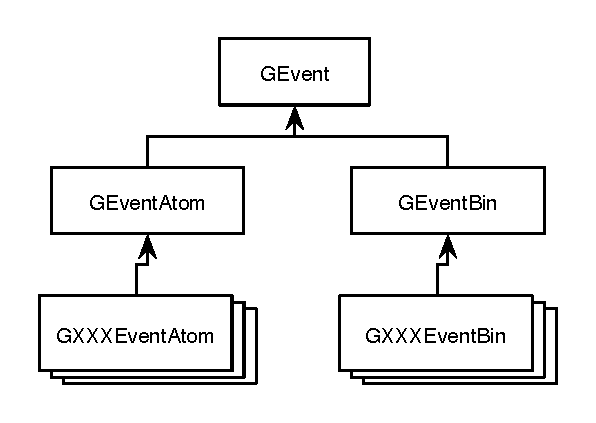
\includegraphics[width=9.1cm]{GEvent.eps}
\caption{Class dependencies for the {\tt GEvent} class.}
\label{fig:GEvent}
\end{figure}
%

The following generic methods are implemented for {\tt GEvent}:
\begin{verbatim}
  std::string string(void);                    //!< Convert event information into string
\end{verbatim}

The {\tt GEventAtom} class contains the following generic event attributes:
\begin{verbatim}
  GTime    m_time;         //!< Time tag of event
  double   m_energy;       //!< Energy of event in MeV
  GSkyDir  m_dir;          //!< Arrival direction of event in sky coordinates
\end{verbatim}

%%%%%%%%%%%%%%%%%%%%%%%%%%%%%%%%%%%%%%%%%%%%%%%%%%%
\subsubsection{{\tt GEvents}}

The basic element of event handling is the {\tt GEvents} abstract container base class that
contains {\tt GEvent} objects.
The derived abstract container class {\tt GEventList} holds {\tt GEventAtom} objects, 
while the derived abstract container class {\tt GEventCube} holds {\tt GEventBin} objects.
Derived from these two classes are the instrument specific container classes
{\tt GXXXEventList} and {\tt GXXXEventCube} (where {\tt XXX} is the instrument code)
which implement the instrument specific methods.
The class dependencies are shown in Fig.~\ref{fig:GEvents}.
%
%
\begin{figure}[!h]
\centering
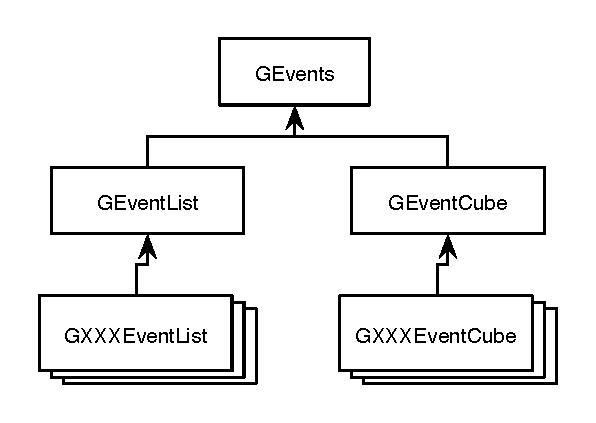
\includegraphics[width=9.1cm]{GEvents.eps}
\caption{Class dependencies for the {\tt GEvents} class.}
\label{fig:GEvents}
\end{figure}
%
%
The following generic methods are implemented:
\begin{verbatim}
  void    load(const std::string& filename);   //!< Load events from FITS file
  void    load(GFitsHDU* hdu);                 //!< Load events from FITS HDU
  GEvent* pointer(int index) const;            //!< Returns pointer to event (atom or bin)
  int     number(void) const;                  //!< Returns total number of events
  int     elements(void) const;                //!< Returns total number of elements
\end{verbatim}
Note that for an event list the total number of elements is identical to the total
number of events.

{\tt GEvents} allows for iterating to provide successive access to events.
The example below shows how iterating is implemented (illustrated using
the {\tt GLATEvents} derived class):
\begin{verbatim}
  GLATEvents events;
  ...
  for (GLATEvents::iterator event = events.begin(); event != events.end(); ++event) {
      cout << *event << endl;
  }
\end{verbatim}




%%%%%%%%%%%%%%%%%%%%%%%%%%%%%%%%%%%%%%%%%%%%%%%%%%%
% User Interface Design
%%%%%%%%%%%%%%%%%%%%%%%%%%%%%%%%%%%%%%%%%%%%%%%%%%%
\section{User Interface Design}

%%%%%%%%%%%%%%%%%%%%%%%%%%%%%%%%%%%%%%%%%%%%%%%%%%%
\subsection{Description of the User Interface}


%%%%%%%%%%%%%%%%%%%%%%%%%%%%%%%%%%%%%%%%%%%%%%%%%%%
% Additional Material
%%%%%%%%%%%%%%%%%%%%%%%%%%%%%%%%%%%%%%%%%%%%%%%%%%%
\section{Additional Material}

\end{document} 
